Per rinominare un progetto un utente deve essere iscritto ed autenticato. Per accedere alla pagina di rinominazione di un progetto l'utente deve premere il pulsante azzurro \textbf{My Project} posto in alto a destra sullo schermo. Una volta premuto si caricherà la pagina corrispondente. A questo punto l'utente deve selezionare il progetto da rinominare dalla lista dei progetti in alto a sinistra.
Una volta selezionato il progetto apparirà al centro dello schermo il titolo del progetto scelto, un'immagine di anteprima della prima slide\ped{G} del progetto e sotto a questa un menù. 

\begin{figure}[H] 
	\centering 
	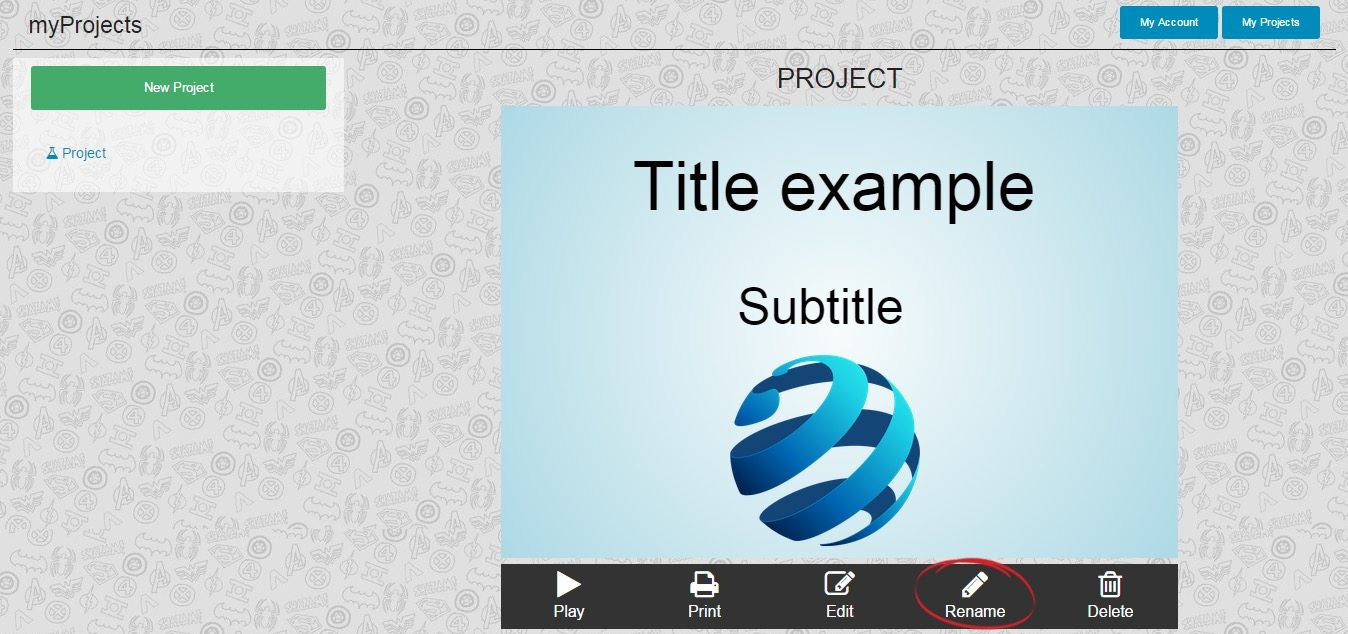
\includegraphics[scale=0.40] {img/rinomina_pro}
	\caption{Rinominazione di un progetto} 
\end{figure}

Selezionando dal menù la voce \textbf{Rename} apparirà il seguente pop-up\ped{G}:

\begin{figure}[H] 
	\centering 
	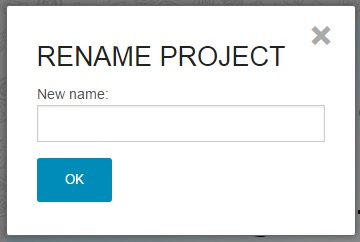
\includegraphics[scale=0.60] {img/rename_project}
	\caption{Pop-up di rinominazione di un progetto} 
\end{figure}

\noindent Per rinominare il progetto sarà sufficiente inserire nell'apposito spazio il nuovo nome che si desidera dare al progetto e successivamente confermare tramite il tasto \textbf{OK}. 